\noindent УДК 519.872

\bigskip
\noindent Р.С.~Хабаров, к.т.н.\par
\noindent В.А.~Лохвицкий, д.т.н.

\begin{center}
{\large\bfseries СВОЕВРЕМЕННОЕ НАЧАЛО ПАКЕТНОГО ОБСЛУЖИВАНИЯ ПРИ НЕТЕРПЕНИИ ЗАЯВОК}
\end{center}

\noindent\textbf{Аннотация.}
Рассматривается одноканальная система с пороговым формированием пакетов, простейшим входящим потоком и экспоненциальным терпением заявок. Распределение времени обслуживания имеет фазовый тип и зависит от размера пакета. По марковской модели ожидания помеченной заявки рассчитываются вероятности своевременного и позднего начала обслуживания, а также ухода без обслуживания. В численных примерах сокращение среднего ожидания среди начавших обслуживание сопровождается уменьшением доли своевременно начавших среди всех поступивших заявок. Показано, что аппроксимация распределения ожидания по двум моментам может изменить выбор максимального размера пакета. Учёт вероятности нулевого ожидания уменьшает общее число ошибок в исследованной серии, но увеличивает число ошибочных признаний параметров допустимыми.

\medskip
\noindent\textbf{Ключевые слова:} пакетное обслуживание, нетерпеливые заявки, помеченная заявка, порог запуска, фазовое распределение, предельное время ожидания.

\begin{center}
\textbf{TIMELY START OF BATCH SERVICE WITH CUSTOMER ABANDONMENT}

R.S.~Khabarov, V.A.~Lokhvitsky
\end{center}

\begin{otherlanguage}{english}
\noindent\textbf{Abstract.}
We consider a single-server queue with threshold-based batch formation, Poisson arrivals and exponential customer patience. Service times have batch-size-dependent phase-type distributions. A Markov model of a tagged customer's waiting process yields the probabilities of timely service start, late service start and abandonment before service. In the numerical examples, a reduction in mean waiting time among customers who enter service accompanies a decrease in the proportion of timely service starts among all arrivals. Two-moment approximations of the waiting-time distribution can change the selected maximum batch size. Preserving the zero-wait probability reduces the total number of errors in the experiments considered but increases false acceptance of infeasible parameter choices.

\medskip
\noindent\textbf{Keywords:} bulk service, abandonment, tagged customer, dispatch threshold, phase-type distribution, deadline.
\end{otherlanguage}

\section*{Введение}

Пакетное обслуживание позволяет распределить затраты на подготовку одной операции между несколькими заявками. Однако накопление пакета увеличивает ожидание, и часть нетерпеливых заявок уходит до начала обслуживания. Среднее время ожидания среди дождавшихся поэтому характеризует лишь часть поступившего потока. Для выбора параметров пакета необходимо знать, какая доля всех заявок начнёт обслуживание в установленный срок.

Основы моделей пакетного обслуживания заложены в работах Bailey и Neuts~\cite{bailey1954,neuts1967}. Время ожидания при пороговом правиле исследовано, в частности, в работах~\cite{medhi1975,claeys2013,chaudhry2023}; зависимость обслуживания от размера пакета учитывается в~\cite{banerjee2015}. Для описания ожидания используем подход с учётом заявок перед помеченной и позади неё~\cite{vanommer2020}. В рассматриваемой модели обслуживание зависит от размера пакета, а уход допускается для всех ожидающих заявок.

Цель работы --- рассчитать вероятность своевременного начала обслуживания и показать, как выбор показателя и приближение распределения ожидания влияют на допустимые параметры пакета. Подробная конструкция цепи, доказательство локальной оценки погрешности и дополнительные проверки вынесены в отдельное приложение.

\section*{Модель и критерии выбора}

Заявки поступают в одноканальную систему простейшим потоком интенсивности $\lambda>0$ и ожидают в неограниченной FIFO-очереди. Свободный канал начинает обслуживание, когда в очереди накоплено не менее $a$ заявок. Из $j$ ожидающих выбираются первые $\min(b,j)$, где $1\leq a\leq b$. Таким образом, $a$ --- порог запуска, $b$ --- максимальный размер пакета. Состав пакета во время обслуживания не меняется; все его заявки завершают обслуживание одновременно.

Время обслуживания пакета размера $i$ обозначим $S_i$. Оно имеет распределение фазового типа: обслуживание проходит через конечное число марковских фаз и завершается поглощением. Закон $S_i$ задаётся отдельно для каждого размера пакета. При запуске нового пакета длительность обслуживания независимо разыгрывается по соответствующему закону.

Время терпения отсчитывается от поступления и имеет распределение $\operatorname{Exp}(\gamma)$ при $\gamma>0$. Если терпение истекло до начала обслуживания, заявка уходит; после его начала уход не допускается. Времена терпения независимы между собой, от входящего потока и случайного выбора длительностей обслуживания. При $\gamma=0$ уходов нет; тогда для устойчивости требуется $\lambda E[S_b]<b$. При положительном $\gamma$ и рассматриваемых конечных фазовых представлениях устойчивость обеспечивается уходом ожидающих заявок.

Выберем поступившую в стационарную систему заявку и назовём её помеченной. Пусть $S$ --- событие начала её обслуживания, $p_S=P(S)$, а $W$ --- время ожидания на этом событии. Для срока $D\geq0$ различаем три исхода: своевременное начало обслуживания с вероятностью $S(D)=P(S,W\leq D)$, позднее начало с вероятностью $L(D)=P(S,W>D)$ и уход без обслуживания с вероятностью $p_A$. Их вероятности удовлетворяют
\begin{equation}\label{eq:outcomes}
 S(D)+L(D)+p_A=1.
\end{equation}

Два естественных требования к своевременности относятся к разным совокупностям заявок. Условный критерий ограничивает долю превысивших срок среди начавших обслуживание. Безусловный учитывает все поступившие заявки, включая ушедшие:
\begin{equation}\label{eq:sla}
 \overline F_S(D)=\frac{L(D)}{p_S}\leq\varepsilon,
 \qquad 1-S(D)=p_A+p_S\overline F_S(D)\leq\varepsilon.
\end{equation}
Здесь $p_S>0$, $\overline F_S$ --- условная дополнительная функция распределения (ДФР), а $\varepsilon$ --- допустимая вероятность неблагоприятного исхода для выбранного критерия. Уход без обслуживания нарушает второе требование независимо от длительности ожидания. В обоих случаях срок относится к началу обслуживания.

\section*{Расчёт вероятностей}

Чтобы проследить ожидание помеченной заявки, учитываем числа заявок перед ней и позади неё, режим канала, размер текущего пакета и фазу обслуживания. Число ожидающих позади существенно: эти заявки помогают достичь порога запуска, но могут уйти до его достижения. Наблюдение заканчивается при начале обслуживания помеченной заявки или её уходе. Получается цепь Маркова с непрерывным временем и двумя видами поглощения.

Начальные веса определяются стационарными вероятностями системы: при простейшем входящем потоке поступающие заявки наблюдают временные доли состояний (свойство PASTA). Вероятность немедленного начала обслуживания обозначим $p_0$. Остальные веса образуют вектор $\alpha$, который не нормируется к единице. Пусть $T$ --- подгенератор продолжающегося ожидания, $s$ --- столбец интенсивностей начала обслуживания и $h=(-T)^{-1}s$. Для конечной цепи стандартные формулы поглощения дают
\begin{align}
 p_S&=p_0+\alpha h, & L(D)&=\alpha e^{TD}h,\label{eq:ph1}\\
 S(D)&=p_S-L(D), & p_A&=\gamma\alpha(-T)^{-1}\mathbf1.\label{eq:ph2}
\end{align}
Столбец $\mathbf1$ состоит из единиц. Эти формулы точны для выбранной конечной цепи; расчёт исходной системы с неограниченной очередью требует усечения. Если исключены начальные состояния суммарного веса $\delta$, полученные вероятности имеют общую массу $1-\delta$, а отброшенный вес учитывается отдельно.

Для усечения по числу заявок позади помеченной получена локальная оценка погрешности вероятностей и ненормированных моментов при фиксированном начальном распределении. Она не включает погрешность стационарных весов. Построение матриц, оценка и её доказательство приведены в приложении.

\section*{Численные результаты}

В примерах среднее время обслуживания равно $g(i)=0{,}1438i+1{,}8874$. Коэффициенты взяты из работы Inoue~\cite{inoue2021} и используются как параметры расчётного примера; время выражено в условных единицах. Сравниваются распределение Эрланга $E_3$ и гиперэкспоненциальное $H_2$ с коэффициентом вариации $1{,}5$ при одинаковом среднем $g(i)$.

\noindent\textbf{Малое среднее ожидание и своевременное обслуживание.}
Рассмотрим $\lambda=0{,}8$, $a=2$, $b=8$, $D=5$ и рост интенсивности ухода от $\gamma=0$ до $0{,}5$. При $E_3$-обслуживании среднее ожидание среди начавших обслуживание уменьшается с $1{,}3244$ до $0{,}6581$, а вероятность своевременного начала для произвольной поступившей заявки --- с $0{,}9797$ до $0{,}6276$. Для $H_2$ последняя вероятность снижается с $0{,}8177$ до $0{,}5772$ (рисунок~\ref{fig:outcomes}).

\begin{figure}[htbp]\centering
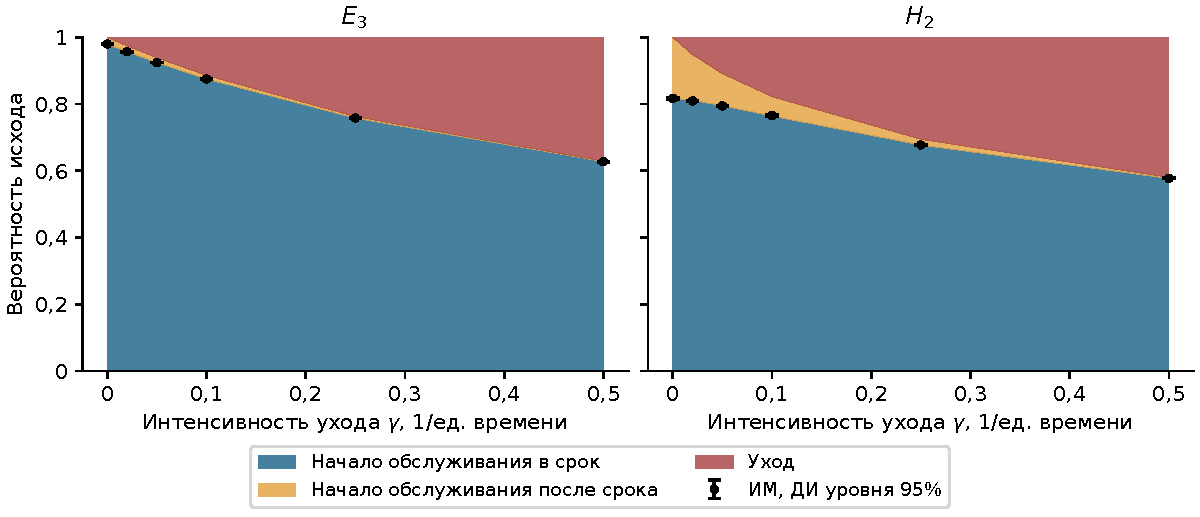
\includegraphics[width=\linewidth]{../figures/revision_outcomes.pdf}
\caption{Три исхода для поступившей заявки при $D=5$, $\lambda=0{,}8$, $a=2$, $b=8$. Точки и интервалы --- оценки вероятности своевременного начала по имитационному моделированию с доверительным уровнем 95\%.}\label{fig:outcomes}
\end{figure}

Уход сокращает очередь и одновременно меняет состав заявок, дождавшихся обслуживания. Поэтому уменьшение условного среднего не означает роста своевременности для всего потока. На рисунке~\ref{fig:feasible} показано, насколько различаются допустимые параметры при двух требованиях. В данном примере область, допустимая по условному критерию, содержит множество настроек, не удовлетворяющих безусловному.

\begin{figure}[htbp]\centering
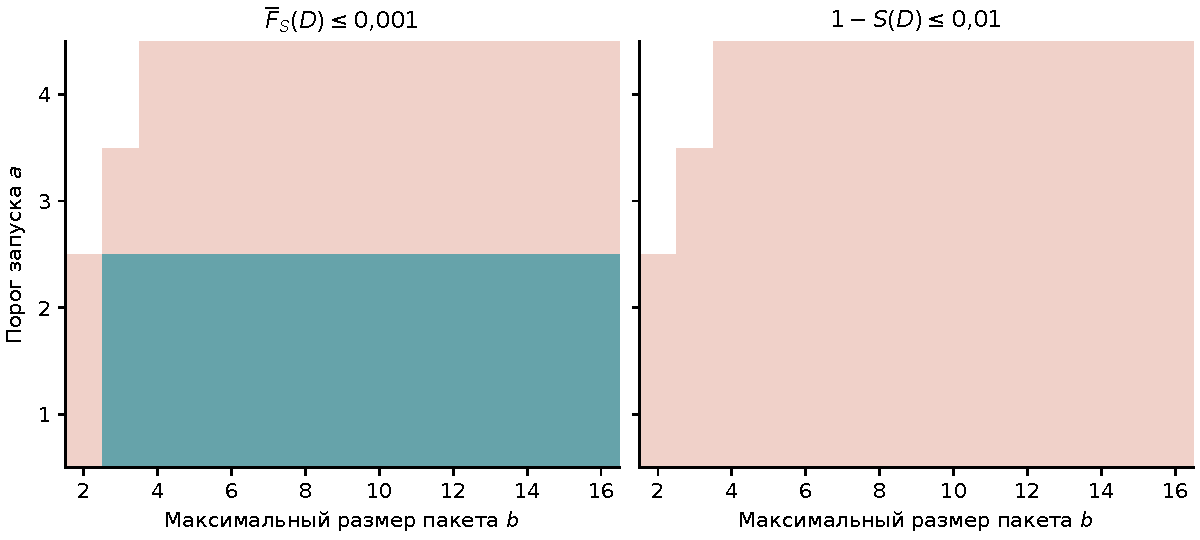
\includegraphics[width=\linewidth]{../figures/revision_feasible.pdf}
\caption{Допустимые параметры при $E_3$-обслуживании, $\lambda=0{,}8$, $\gamma=0{,}1$, $D=10$. Слева проверяется $\overline F_S(D)\leq0{,}001$, справа --- $1-S(D)\leq0{,}01$. Синий цвет означает выполнение требования, розовый --- нарушение; белые клетки соответствуют $a>b$.}\label{fig:feasible}
\end{figure}

\noindent\textbf{Аппроксимация ожидания и выбор размера пакета.}
Сравним расчёт по марковской модели с двумя приближениями условного распределения ожидания. Первое --- гамма-распределение, подобранное по первым двум начальным моментам. Во втором сохраняется вероятность нулевого ожидания $z=p_0/p_S$, а гамма-распределением приближается только положительное ожидание. В таблицах эти варианты названы «Гамма» и «Атом + гамма»: атом в нуле означает положительную вероятность немедленного начала обслуживания. Моменты и $p_S$ в обоих приближениях берутся из марковского расчёта; сравнение выделяет влияние формы распределения.

Исследованы 228 вариантов: $\lambda=0{,}8$, $b=2,\ldots,16$, $a=1,\ldots,\min(4,b)$, законы $E_3$ и $H_2$, $\gamma=0;0{,}1$. Для сроков $D=5,10,20$ и трёх допусков каждого критерия выполнено по 2052 проверки. Ошибочное признание допустимости означает, что приближение принимает параметры, отклоняемые расчётом по марковской модели; ошибочное отклонение --- обратное несоответствие. Различия с порогом до $10^{-7}$ включительно считаются неразличимыми; таких случаев в серии нет.

\begin{table}[htbp]\centering\small
\caption{Ошибки проверки допустимости: 2052 проверки для каждого критерия и приближения}\label{tab:decisions}
\begin{tabular}{p{.17\linewidth}p{.21\linewidth}p{.17\linewidth}p{.15\linewidth}p{.16\linewidth}}
\hline
Критерий & Аппроксимация & Ошибочное признание допустимости & Ошибочное отклонение & Неразличимо \\
\hline
Условный & Гамма & 20 & 61 & 0 \\
Условный & Атом + гамма & 34 & 20 & 0 \\
Безусловный & Гамма & 1 & 6 & 0 \\
Безусловный & Атом + гамма & 1 & 3 & 0 \\
\hline
\end{tabular}

\end{table}

Для условного критерия учёт нулевого ожидания уменьшил общее число ошибок с 81 до 54, но увеличил число ошибочных признаний допустимости с 20 до 34 (таблица~\ref{tab:decisions}). Следовательно, в исследованной серии уменьшение общего числа ошибок не сделало выбор более осторожным.

Практическое следствие видно на двух примерах в таблице~\ref{tab:choices}. При $D=10$ и $\varepsilon=0{,}001$ расчёт требует $b=5$, а вариант «Атом + гамма» допускает $b=4$. При $\varepsilon=0{,}0001$ расчёт даёт $b=10$, но оба приближения отклоняют все значения до 16. Минимум ищется перебором всех целых $b$ в заданном диапазоне при фиксированных остальных параметрах; монотонность вероятности по $b$ не предполагается.

\begin{table}[htbp]\centering\small
\caption{Примеры выбора наименьшего допустимого $b\in\{2,\ldots,16\}$ по условному критерию: $E_3$, $a=1$, $\lambda=0{,}8$, $\gamma=0$, $D=10$. Прочерк --- отсутствие допустимого значения в этом диапазоне}\label{tab:choices}
\begin{tabular}{rrrr}
\hline
$\varepsilon$ & Расчёт & Гамма & Атом + гамма \\
\hline
0,001 & 5 & 5 & 4 \\
0,0001 & 10 & --- & --- \\
\hline
\end{tabular}

\end{table}

\noindent\textbf{Проверка и границы численных выводов.}
Стационарное усечение увеличивалось до выполнения двух условий: вероятность граничных состояний не выше $10^{-10}$ и изменение первых двух моментов и вероятностей не выше $10^{-7}$. Критерий выполнен для всех 12 вариантов исследования нетерпения и всех 228 вариантов выбора параметров. Он служит численной диагностикой, а не оценкой полной погрешности. Во вспомогательной серии по нагрузке три варианта с $H_2$ не удовлетворили критерию даже при границе 1600 и исключены из соответствующего сопоставления; подробности сохранены в приложении.

Для 12 вариантов по нетерпению проведено по 12 независимых имитационных повторений: 100\,000 учитываемых заявок после 20\,000 поступлений переходного периода. Доверительные интервалы уровня 95\% построены по распределению Стьюдента на основе повторений и относятся к отдельным величинам. Два из 36 сопоставлений находятся вне своих интервалов. Малые хвостовые вероятности не считаются подтверждёнными этой имитацией; их расчёт опирается на марковскую схему и проверку численной сходимости.

\section*{Заключение}

Для системы с нетерпеливыми заявками выбор параметров пакета должен учитывать своевременное и позднее начало обслуживания, а также уход. Рассмотренные примеры показывают, что условное среднее ожидания может уменьшаться одновременно со снижением доли своевременно начавших обслуживание среди всех поступивших заявок.

Аппроксимации по двум моментам способны как принять недопустимые параметры, так и отклонить допустимые. Сохранение вероятности нулевого ожидания не устранило эти ошибки и в исследованной серии увеличило число ошибочных допусков. Расчёт вероятностей по марковской модели позволяет проверять выбранный критерий непосредственно и находить допустимые параметры перебором в заданном диапазоне с контролем численной сходимости.

Реализация доступна в библиотеке most-queue~\cite{mostqueue2026}. Приложение содержит подробности метода, доказательство локальной оценки и дополнительные численные результаты; протокол, данные и материалы воспроизведения сохранены в вычислительном комплекте статьи.
